\documentclass[border=20pt]{standalone}

\usepackage{tikz}
\usepackage{ifthen}
\usetikzlibrary{arrows, positioning, calc}
\usetikzlibrary{shapes.multipart} 

\usepackage{incgraph}
\usepackage{standalone}
\begin{document}
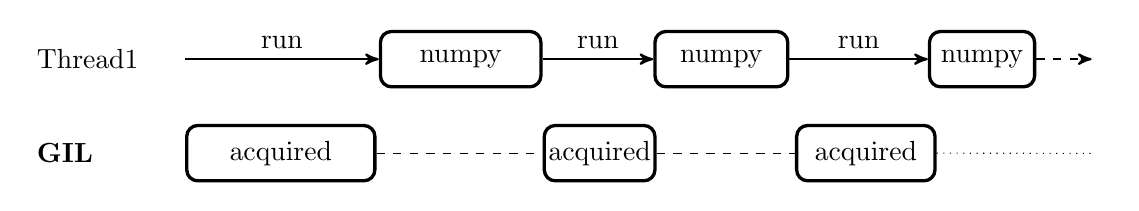
\begin{tikzpicture}

\def\iotext{numpy}

\tikzset{
    %Define standard arrow tip
    >=stealth',
    %Define style for boxes
    rbox/.style={
           rectangle,
           fill=white,
           rounded corners,
           draw=black, very thick,
           text width=2em,
           minimum height=2em,
           text centered},
    run/.style={
           ->,
           thick
    },
    wait/.style={
           dotted,
           thick
    },
};

%nodes

\node[text width=5em] (thread1) {Thread1};
\node[rbox, right=7em of thread1, text width=6em, inner sep=-0.1em] (io1) {\iotext};
\draw[run] (thread1.east) -- (io1.west) node[midway, above]  {run};
\node[rbox, right=4em of io1, text width=5em, inner sep=-0.1em] (io2) {\iotext};
\path (io1.east) edge[run] node[midway, above]  {run} (io2.west) ;
\node[rbox, right=5em of io2, text width=4em,  inner sep=-0.1em] (io3) {\iotext};
\path (io2.east) edge[run] node[midway, above]  {run} (io3.west) ;
\node[right=2em of io3] (end1) {};
\path (io3.east) edge[run, dashed] (end1);

\node[below=2em of thread1, text width=5em] (gil) {\bf GIL};
\node[rbox, right=0em of gil, text width=7em, inner sep=-0.1em] (lock1) {acquired};
\node[rbox, right=6em of lock1, text width=4em, inner sep=0em] (lock2) {acquired};
\node[rbox, right=5em of lock2, text width=5em, inner sep=0em] (lock3) {acquired};
\node[below=2.7em of end1] (end2) {};
\path (lock1.east) edge[dashed] (lock2.west);
\path (lock2.east) edge[dashed] (lock3.west);
\path (lock3.east) edge[dotted] (end2);

% Draw a centered plus sign

\end{tikzpicture}
\end{document}